\section*{Limitations}
% not work well in huge compression ratio
% tokenizer are difference, between small LLM and black-box LLMs, 尤其是LLaMdA的tokenizer对于多语言支持较差

% \paragraph{Upperbound of Compression Ratio}
There are also some limitations in our approach.
For instance, we might observe a notable performance drop when trying to achieve excessively high compression ratios such as 25x-30x on GSM8K, 
% a significant performance drop may occur under excessively high compression ratios, such as over 25x-30x for GSM8K,
as shown in Figure~\ref{fig:big_compression_atio}.
\begin{figure}[htb]
    \centering
    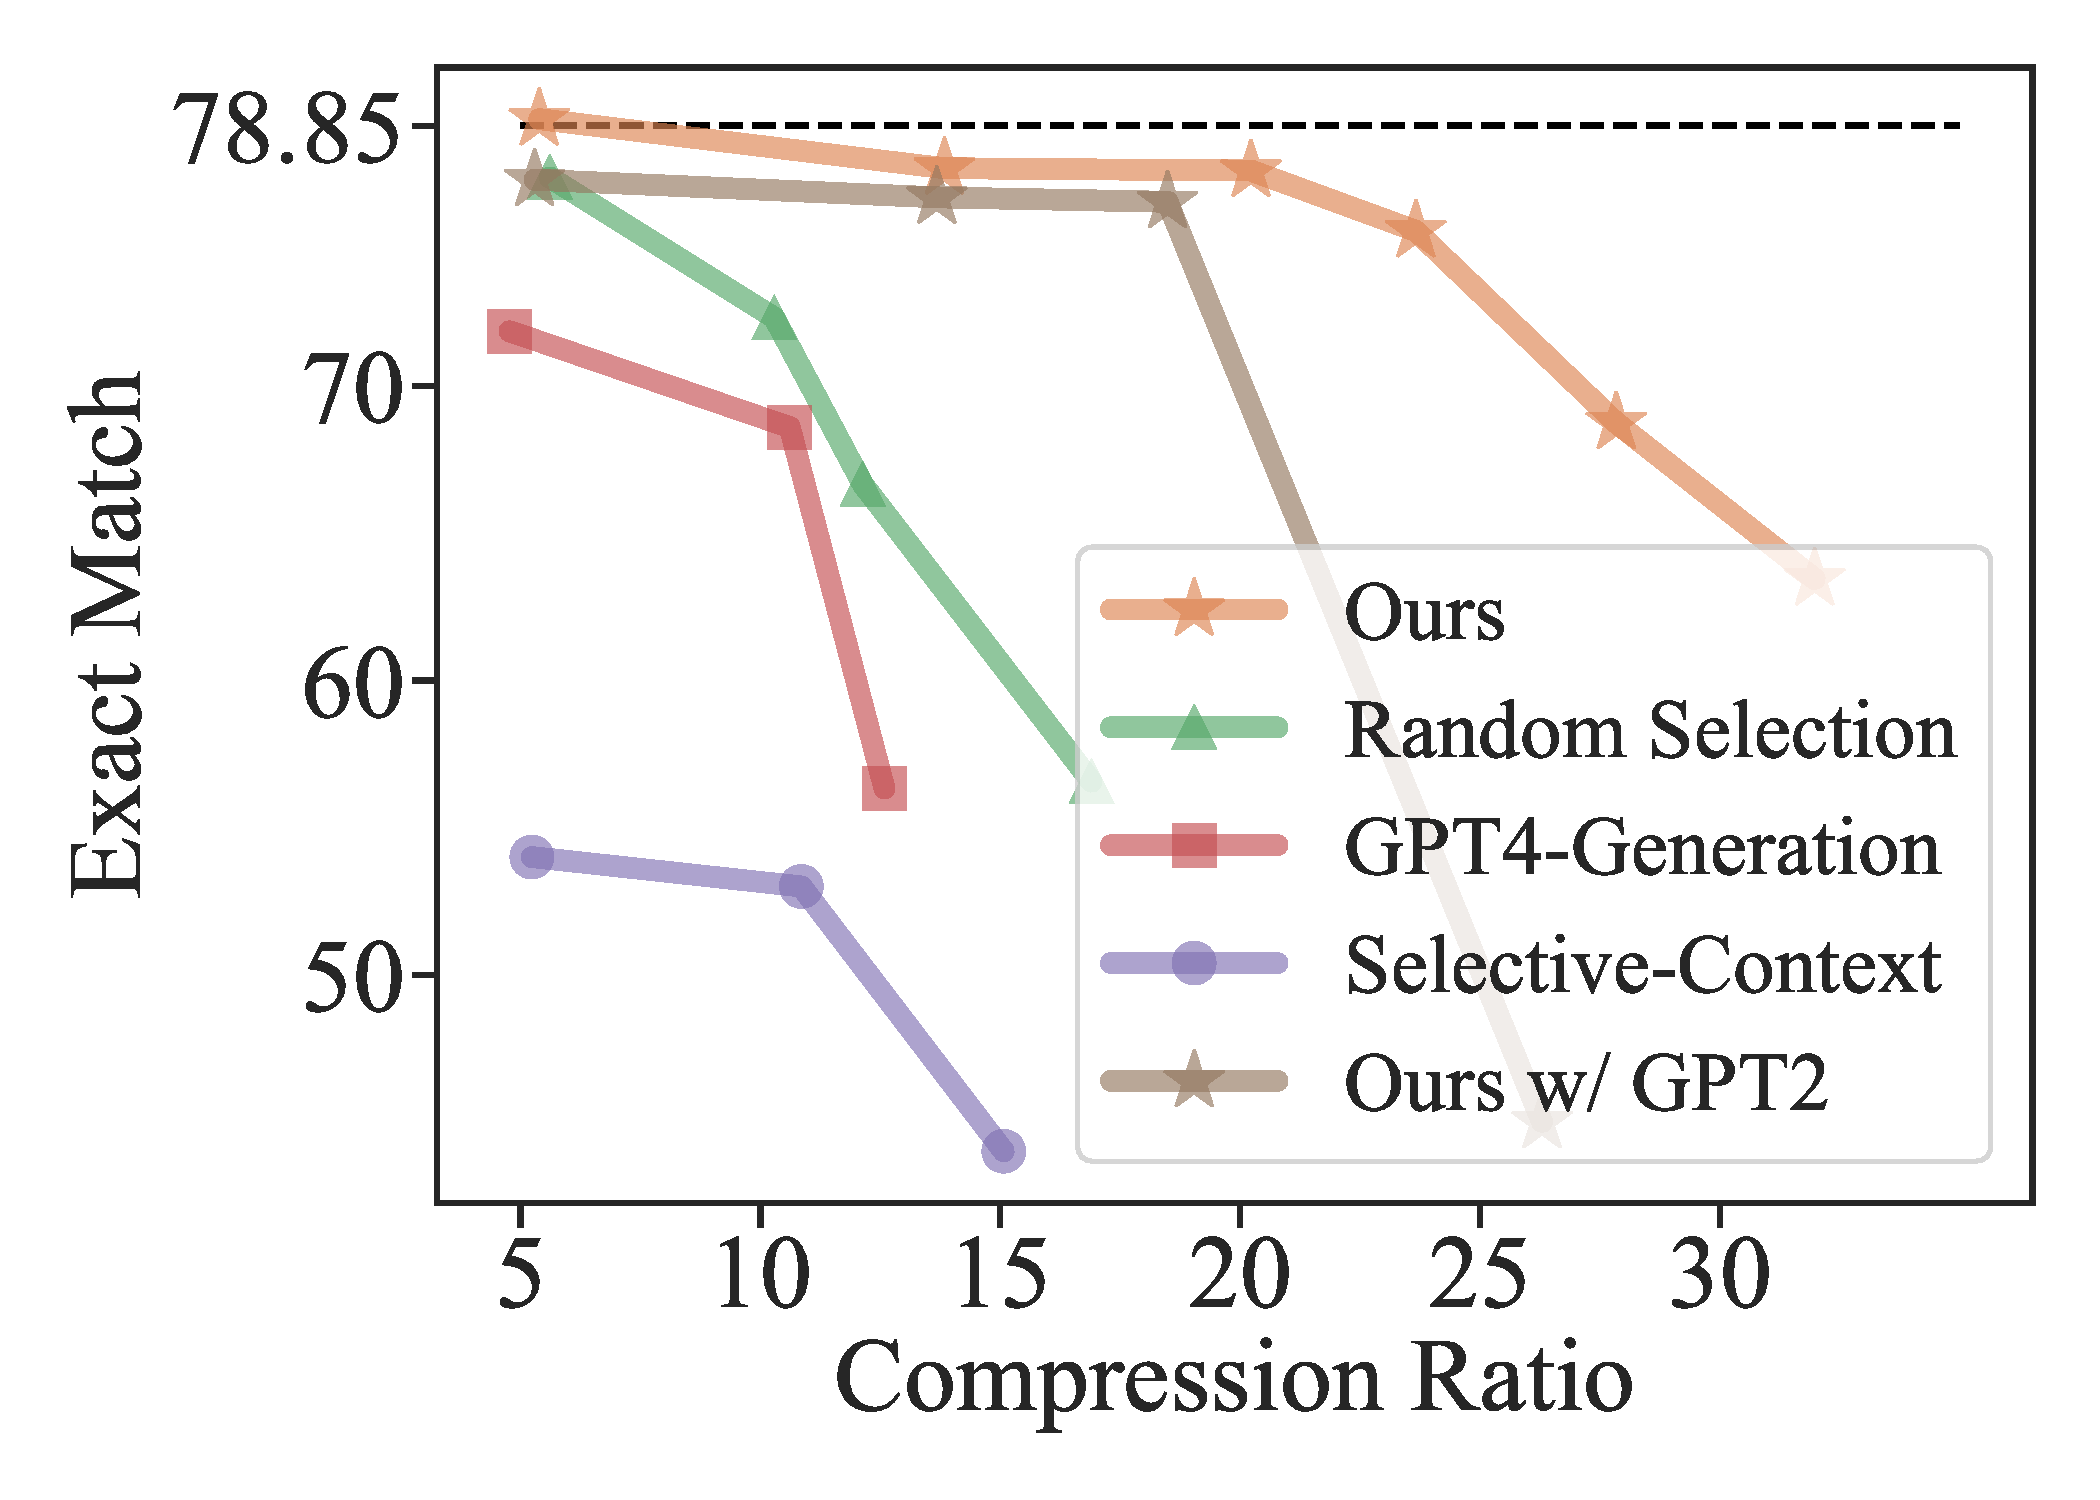
\includegraphics[width=\linewidth]{figures/compression_ratio_performance_gsm8k.pdf}
    \caption{The performance of various prompt compression methods at different compression ratios ($1/\tau$) on GSM8K. The dashed line corresponds to the Exact Match score obtained from the full-shot prompt.}
    \label{fig:big_compression_atio}
\end{figure}

It is shown that
% It can be observed that 
as the compression ratio increases especially around 25x-30x, all methods as well as ours will experience a substantial performance drop.
In comparison with other methods, this performance drop derived from our approach is significantly shifted to much higher compression ratios. 
We owe this to the Budget Controller and the Iterative Token-level Prompt Compression algorithm, which enable our method to maintain the original prompt information even at some extreme compression ratios.
The upper limit of the compression ratio for different prompts varies, depending on factors such as prompt length, task type, and the number of sentences involved.

Additionally, there may be subtle differences between the tokenizers used by the small language model and the black-box LLM, which may result in an underestimation of the prompt's token length.
% the prompt token length compared to the actual token length.

% As shown in Figure~\ref{fig:big_compression_atio}, we also conducted tests at higher compression ratios. It can be observed that as the compression ratio further increases, even our method experiences a noticeable performance drop around 25x-30x. In comparison with other methods, this performance drop is significantly shifted to the right, thanks to the Budget Controller and Iterative Token-level Prompt Compression, which enable our method to maintain the original prompt information even at more extreme compression ratios. The upper limit of the compression ratio for different prompts varies, depending on factors such as prompt length, task type, and the number of sentences.

% Our methods also have some limitations. For instance, a significant performance drop may occur under excessively high compression ratios, such as over 25x-30x for GSM8K. Additionally, there may be subtle differences between the tokenizer of the small language model and that of the black-box language model, which could lead to underestimation of the prompt token length compared to the actual token length.